\documentclass{beamer}
%~ \usetheme{Hannover}  %% Themenwahl
%~ \usetheme{Bergen}  %% Themenwahl
\usetheme{Berkeley}  %% Themenwahl
\usecolortheme{dove}

\usepackage[utf8]{inputenc}
\usepackage[T1]{fontenc}

\usepackage[english]{babel}

\usepackage{graphicx}
\usepackage{upgreek}
\usepackage{float}
\usepackage{units}
\usepackage{url}

\usepackage{amsmath}
\usepackage{amssymb}
\usepackage{amsfonts}

\usepackage{longtable}

\usepackage{ae}
\usepackage{booktabs}

\usepackage{tikz}
\usetikzlibrary{patterns}

%\abs{Ausdruck} %Betragsstriche, die skalieren - abgekürzt
\newcommand{\abs}[1]{\ensuremath{\left\vert#1\right\vert}}
% und das gleiche füur große Klammern
\newcommand{\brac}[1]{\ensuremath{\left(#1\right)}}
% Erwartungswert skalierend
\newcommand{\avg}[1]{\left< #1 \right>}
% ein nicht kursives d für Ableitungen/Integrale, mit etwas Platz davor, um sich etwas abzusetzten
\newcommand{\de}{\ensuremath{\,\mathrm{d}}}
% Für Einheiten: schreibt sie nicht kursiv und lässt etwas Platz zur Zahl vorher
\newcommand{\eh}[1]{\ensuremath{\,\mathrm{#1}}}
% einfaches Gradzeichen
\newcommand{\gr}{\ensuremath{^{\circ}}}
% Fehlerfortpfanzung
% dy/dz * delta z
\newcommand{\fehler}[2]%
{\ensuremath{\abs{\frac{\partial #1}{\partial #2}}\cdot \Delta #2}}

\title{Ising-Ferromagnet auf Ad-Hoc Netzwerken}
\author{Hendrik Schawe}
\date{\today}

\begin{document}

\maketitle
\frame{\tableofcontents[pausesections]}

\section{Model}
    \subsection{Ising Ferromagnet}
        \begin{frame}{Ising Ferromagnet}
            \begin{itemize}[<+->]
                \item \(N\) sites
                \item \(\avg{i,j}\) denotes "nearest neighbor" relationship
                \item every site has a spin \(s \in \{-1,+1\}\){}
                \item two spins \(i,j\) are coupled by \(J_{i,j}\){}
                \item{
                    \begin{equation}
                        H = - \sum_{\avg{i,j}}J_{ij}s_{i}s_{j}.
                    \end{equation}
                    (Ref.\ \cite{Ising1925})
                }
            \end{itemize}
        \end{frame}

        \begin{frame}{Disordered Ising Ferromagnet}
            \begin{columns}[t]
                \begin{column}{5cm}
                    \begin{itemize}
                        \item start with square lattice
                        \pause
                        \item displace every node randomly according to\\
                            \(f(x)=\frac{1}{\sqrt{2\pi}\sigma}\mathrm{e}^{-\frac{x^2}{2\sigma^2}}.\)
                    \end{itemize}
                \end{column}
                \begin{column}{6cm}
                    \vspace{-1cm}
                    \begin{figure}[htbp]
                        \centering
                        \begin{tikzpicture}[scale=1.5, declare function={
        normal(\x,\m,\y) = 1/exp((\x-\m)*(\x-\m)/2/(\s^2))-\y;
      }]
    \def\s{0.5}

    \draw[dashed] (-2,0) -- (4,0);
    \draw[dashed] (0,-2) -- (0,2);
    \draw[dashed] (2,-2) -- (2,2);

    \def\dxa{0.4}
    \def\dya{-0.8}

    \draw (\dxa,\dya) -- node [below] {$\Delta x$} (0,\dya);
    \draw (\dxa,\dya) -- node [right] {$\Delta y$} (\dxa,0);
    \draw[loosely dotted] (\dxa,0) -- (\dxa,{1.6+normal(\dxa,0,0)});
    \draw[loosely dotted] (0,\dya) -- ({-1.6-normal(\dya,0,0)},\dya);
    \draw[->] (0,0) -- (0+\dxa*0.9,0+\dya*0.9);

    \draw[color=black,domain=-1.5:1.5] plot [smooth] (\x,{normal(\x,0,0)+1.6}) node[right] {};
    \fill (0, 0) circle(0.08);
    \draw[color=black] (0+\dxa, 0+\dya) circle(0.08);
    \draw[color=black,domain=-1.5:1.5,rotate=90] plot [smooth] (\x,{normal(\x,0,0)+1.6}) node[right] {};

    \draw[|-|] (-\s,2.8) -- node [above] {$\sigma$} (\s,2.8);
    \draw[|-|] (-2.8,-\s) -- node [left] {$\sigma$} (-2.8,\s);


    \def\dxb{0.5}
    \def\dyb{0.2}

    \draw[color=gray] (2+\dxb,0+\dyb) -- node [above] {$\Delta x_{2}$} (2, \dyb);
    \draw[color=gray] (2+\dxb,0+\dyb) -- node [right] {$\Delta y_{2}$} (2+\dxb,0);
    \fill[color=gray] (2, 0) circle(0.08);
    \draw[color=gray] (2+\dxb, 0+\dyb) circle(0.08);
\end{tikzpicture}

                        \caption
                        {
                            Displacement of the nodes.
                        }
                    \end{figure}
                \end{column}
            \end{columns}
        \end{frame}

    \subsection{Proximity Graphs}
        \begin{frame}{Proximity Graphs}
            \begin{itemize}[<+->]
                \item{ 3 graph types used
                    \begin{itemize}
                        \item Delaunay Triangulation (DT) \cite{Katajainen}
                        \item Gabriel Graph (GG) \cite{Gabriel1969}
                        \item Relative Neighborhood Graph (RNG) \cite{Toussaint1980}
                    \end{itemize}
                }
                \item{
                    \begin{equation}
                        DT \supseteq GG \supseteq RNG
                    \end{equation}
                }
            \end{itemize}
        \end{frame}

        \begin{frame}{Delaunay Triangulation}
            \begin{figure}[htbp]
                \centering
                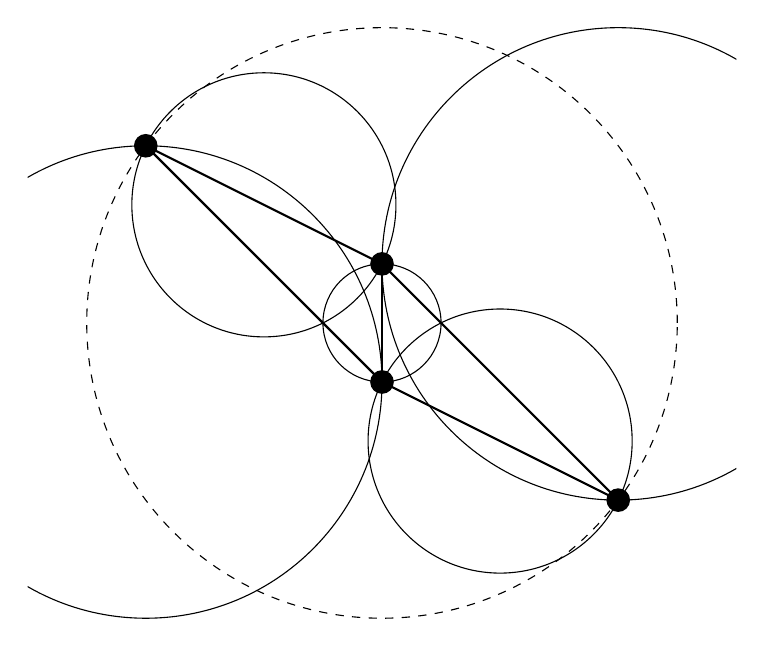
\begin{tikzpicture}[scale=3]
    \clip (-0.5,0) rectangle (2.5,2.5);

    \fill (0, 2  ) circle(0.05);
    \fill (1, 1.5) circle(0.05);
    \fill (1, 1  ) circle(0.05);
    \fill (2, 0.5) circle(0.05);

    \draw[dashed] (1, 1.25)   circle(1.25);
    \draw (2, 1.5)      circle(1);
    \draw (1, 1.25)     circle(0.25);
    \draw (0.5, 1.75)   circle(0.5590);
    \draw (1.5, 0.75)   circle(0.5590);
    \draw (0, 1)        circle(1);

    \draw[thick] (0, 2  ) -- (1, 1.5);
    \draw[thick] (0, 2  ) -- (1, 1  );
    \draw[thick] (1, 1  ) -- (1, 1.5);
    \draw[thick] (1, 1  ) -- (2, 0.5);
    \draw[thick] (1, 1.5) -- (2, 0.5);
\end{tikzpicture}

                \caption
                {
                    Example of a DT.
                }
            \end{figure}
        \end{frame}

        \begin{frame}{Gabriel Graph}
            \begin{columns}[b]
                \begin{column}{5cm}
                    \begin{figure}[htbp]
                        \centering
                        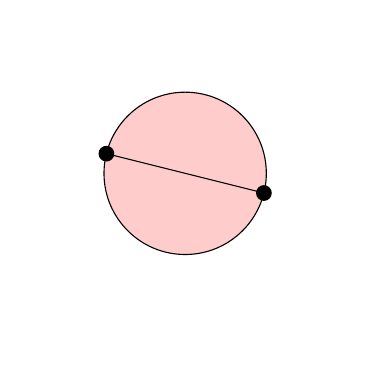
\begin{tikzpicture}
    \clip (-2,2.1) rectangle (2,-2);

    \fill[fill=red!20] (0, 0.25) circle(1.0307764064);
    \draw (0, 0.25) circle(1.0307764064);
    %~ \pattern[pattern color=black!60, pattern=north west lines];


    \fill (-1, 0.5) circle(0.1);
    \fill (1, 0) circle(0.1);
    \draw (1, 0) -- (-1, 0.5);
\end{tikzpicture}

                        \caption
                        {
                            Lune of a GG.
                        }
                    \end{figure}
                \end{column}
                \begin{column}{5cm}
                    \begin{figure}[htbp]
                        \centering
                        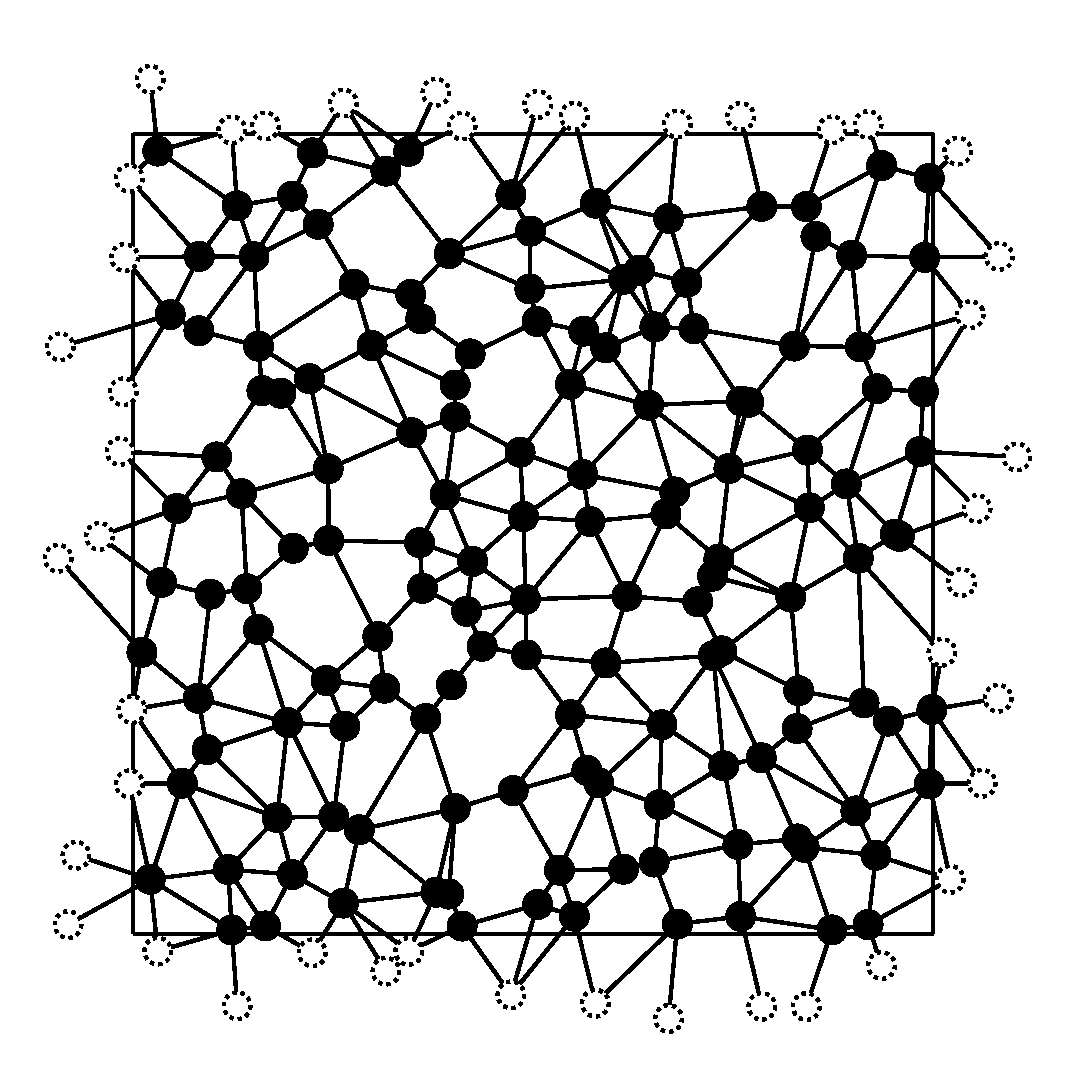
\includegraphics[width=1\textwidth]{images/GG/L12S03.pdf}
                        \caption
                        {
                            GG Example
                        }
                    \end{figure}
                \end{column}
            \end{columns}
        \end{frame}

        \begin{frame}{Relative Neighborhood Graph}
            \begin{columns}[b]
                \begin{column}{5cm}
                    \begin{figure}[htbp]
                        \centering
                        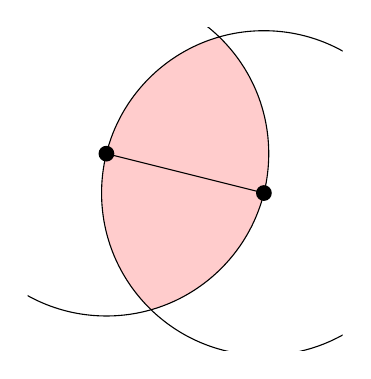
\begin{tikzpicture}
    \clip (-2,2.1) rectangle (2,-2);
    % Shade the intersection where signals collide.
    \begin{scope}
        \clip (-1, 0.5) circle(2.06155281281);
        \fill[fill=red!20] (1, 0) circle(2.06155281281);
    \end{scope}

    \draw (-1, 0.5) circle(2.06155281281);
    \fill (-1, 0.5) circle(0.1);
    \draw (1, 0) circle(2.06155281281);
    \fill (1, 0) circle(0.1);
    \draw (1, 0) -- (-1, 0.5);
\end{tikzpicture}

                        \caption
                        {
                            Lune of a RNG.
                        }
                    \end{figure}
                \end{column}
                \begin{column}{5cm}
                    \begin{figure}[htbp]
                        \centering
                        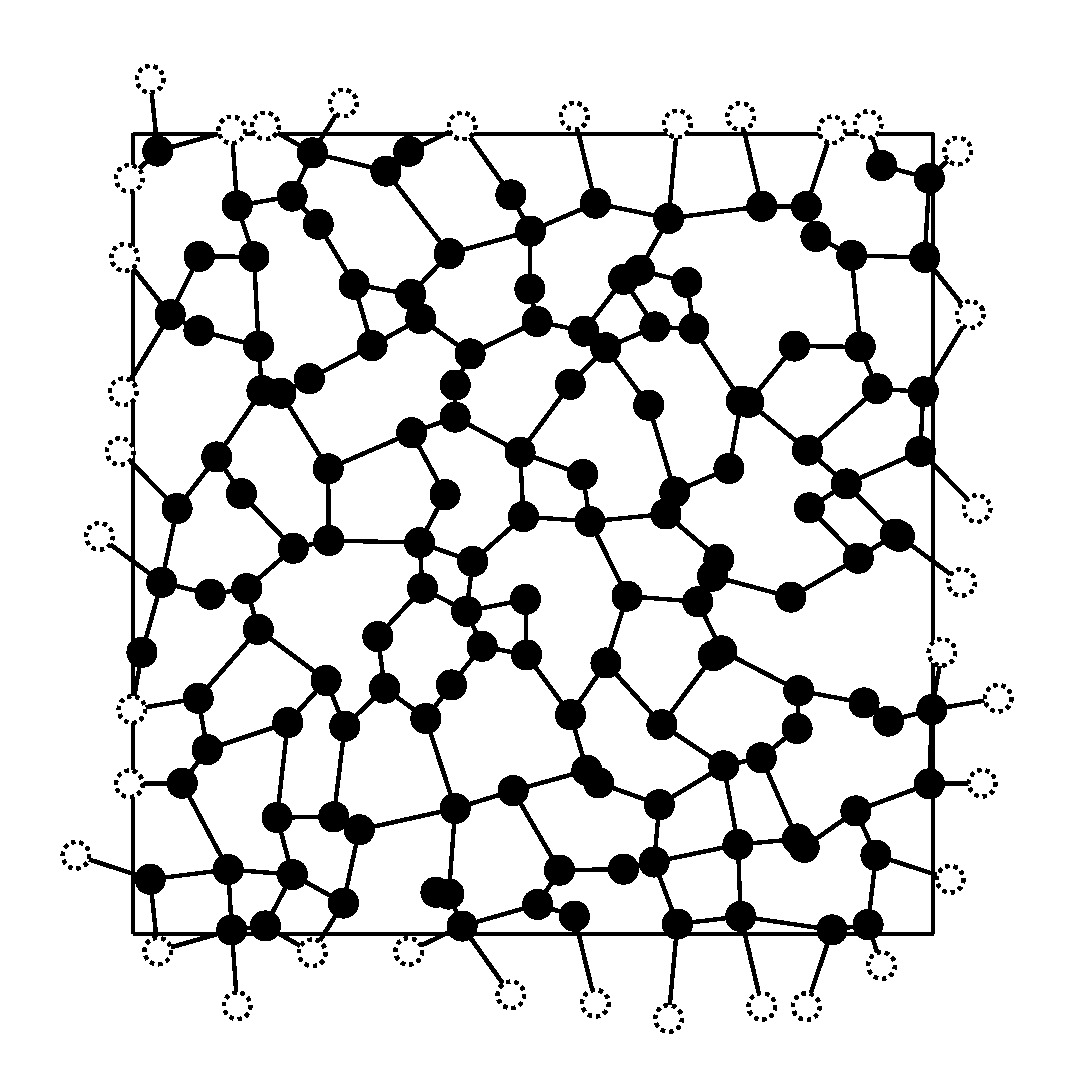
\includegraphics[width=1\textwidth]{images/RNG/L12S03.pdf}
                        \caption
                        {
                            RNG Example
                        }
                    \end{figure}
                \end{column}
            \end{columns}
        \end{frame}

\section{Methods}
    \subsection{Monte Carlo Simulations}
        \begin{frame}{Monte Carlo Simulations}
            \begin{itemize}[<+->]
                \item generate random states
                \item mesure observables of these states
                \item{ estimate observable \(O\) by
                    \begin{equation}
                        \avg{O} = \frac{1}{Z} \sum_i p_i O_i
                    \end{equation}
                }
            \end{itemize}
            \begin{itemize}[<+->]
                \item But there are states contributing more than others
                \item{ e.g.\ low \(H_{i}\) in canonical systems at low \(T\) with
                    \begin{equation}
                        p_{i} = e^{-\frac{H_{i}}{k_{B}T}}
                    \end{equation}
                }
            \end{itemize}
        \end{frame}

        \begin{frame}{Importance Sampling}
            \begin{itemize}[<+->]
                \item generate new states according to the known distribution \(p_{i}\)
                \item generate new states from former states
                \item{ Markov Chains
                    \begin{itemize}
                        \item Ergodicity\\
                                every state is reachable in finite time
                        \item Detailed Balance\\
                                in equilibrium the probability to reach a state is the same as the probability to leave the same state
                    \end{itemize}
                }
                \item note that the correlation of subsequent states has an effect on the errorbars\\
                    \(\to\) autocorrelation time \(\tau\)
            \end{itemize}
        \end{frame}

        \begin{frame}{Single Spin Flip Metropolis Update \cite{Metropolis1953}}
            \begin{equation}
                A(\mu \to \nu) =
                \begin{cases}
                    1                            & \Delta H \le 0 \\
                    \exp{\brac{-\beta \Delta H}} & \Delta H > 0
                \end{cases}.
            \end{equation}
        \end{frame}

        \begin{frame}{Wolff Cluster Update \cite{Wolff1989}}
            \begin{equation}
                P_{\mathrm{add}} = 1-\exp\brac{-2\beta J},
            \end{equation}
            \pause
            \begin{itemize}[<+->]
                \item very efficient at \(T_{c}\)
                \item but inferior to Metropolis at large and small \(T\)
            \end{itemize}
        \end{frame}

        \begin{frame}{Parallel Tempering \cite{ParallelTempering1986}}
            \begin{equation}
                P_{i,i+1}((E_i,T_i) \to (E_{i+1},T_{i+1})) = \min\brac{1,e^{\brac{\brac{E_{i+1}-E_i}\brac{\frac{1}{T_{i+1}}-\frac{1}{T_i}}}}}
            \end{equation}
            \begin{columns}[b]
                \begin{column}{5cm}
                    \begin{figure}[htbp]
                        \centering
                        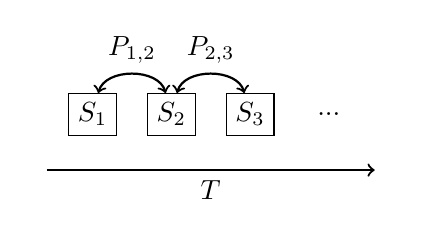
\begin{tikzpicture}
    \node[draw,rectangle] (a) {$S_1$};
    \node[draw,rectangle,right of=a] (b) {$S_2$};
    \node[draw,rectangle,right of=b] (c) {$S_3$};
    \node[rectangle,right of=c] (d) {...};

    \node[rectangle,below left of=a] (A) {};
    \node[rectangle,below right of=d] (D) {};
    \draw[thick,->] (A) edge node[below] {$T$} (D);

    \draw[thick,<->] (a) edge[out=75,in=105] node[above] {$P_{1,2}$} (b);
    \draw[thick,<->] (b) edge[out=75,in=105] node[above] {$P_{2,3}$} (c);
    %~ \draw[thick,<->] (c) edge[out=80,in=100] node[above] {$P_{..}$} (d);
\end{tikzpicture}

                        \caption
                        {
                            Swapping the spin configurations.
                        }
                    \end{figure}
                \end{column}
                \pause
                \begin{column}{6cm}
                    \begin{figure}[htbp]
                        \centering
                        \documentclass{standalone}
\usepackage{tikz}

\begin{document}
    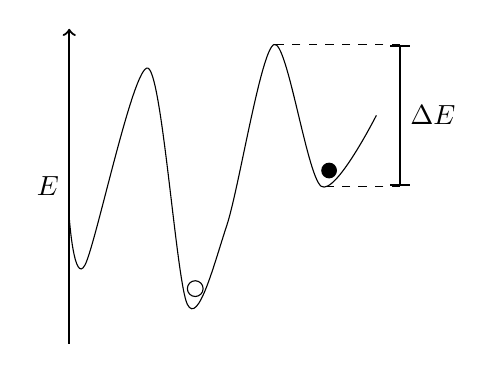
\begin{tikzpicture}
        %~ \draw[thick,->] (0,0) -- node[below] {$T$} (6,0);
        \draw[thick,->] (0,0) -- node[left] {$E$} (0,4);

        \draw plot [smooth] coordinates {(0,1.6) (0.2,1) (1,3.5) (1.5,0.5) (2,1.5) (2.6,3.8) (3.2,2) (3.9,2.9)};

        \fill (3.3,2.2) circle(0.1);
        \draw (1.6,0.7) circle(0.1);

        \draw[thick,|-|] (4.2,2) -- node[right] {$\Delta E$} (4.2,3.8);
        \draw[dashed] (4.2,2) -- (3.2,2);
        \draw[dashed] (4.2,3.8) -- (2.6,3.8);
    \end{tikzpicture}
\end{document}

                        \caption
                        {
                            Sketch of an energy landscape.
                        }
                    \end{figure}
                \end{column}
            \end{columns}
        \end{frame}

\section{References}
    \begin{frame}[allowframebreaks]
        \bibliography{lit}
        \bibliographystyle{amsplain}
    \end{frame}

\end{document}
